\chapter{Andere indices}\label{ch:andere-indices}
Naast suffixbomen en suffix arrays bestaan er ook nog enkele andere interessante indexstructuren.
We behandelen in dit hoofdstuk FM- en R-indices.
Deze maken achterliggend gebruik van suffix arrays, maar zorgen ervoor dat de index zelf kleiner wordt doordat niet de volledige tekst bijgehouden moet worden.


\section{FM-index}
Deze indexstructuur is vernoemd naar Ferragina en Manzini die dit als eerste beschreven hebben~\cite{fm_index}.
Een FM-index bestaat uit 3 essentiële componenten.
De Borrows-wheeler transformatie~\cite{bwt}, een (sparse/compressed) suffix array en bitvectoren die de rank-operatie ondersteunen.
Het opbouwen van de index kan gebeuren in $O(n)$ met $n$ de lengte van de invoertekst.
Het zoeken van een match kan in $O(m)$ (met $m$ de lengte van de zoekstring).
Het zoeken inclusief het vinden van waar alle matches in de originele string zitten kan in $O(m + \text{|occ}(P, T)\text{|} \log n)$.
Hierbij is $\text{occ}(P, S)$ de set van alle string dat prefix $P$ matcht in de input tekst $T$.
Door gebruik te maken van de BWT heeft deze indexstructuur als voordeel dat niet de volledige tekst expliciet bijgehouden moet worden, waar dus een significante winst kan gemaakt worden ten opzichte van het gebruik van enkel een suffix array.
Aan de hand van een variant van de FM-index, de bidirectionele FM-index kan men bovendien gebruikmaken van een techniek om efficiënt inexacte matching, waarbij maximaal $x$ mismatches toegelaten zijn, uit te voeren.
Dit worden zoekschema's genoemd.

\subsection{Verschillende implementaties}
Om een goed beeld te krijgen over het geheugenverbruik tijdens het opbouwen hebben we verschillende bestaande FM-index implementaties getest.
Opnieuw focussen we ons vooral op het geheugenverbruik aangezien dit de primaire restrictie tijdens het opbouwen.
Tabel~\ref{tab:fm_index_building} geef een overzicht van de geteste implementaties.
Omdat ons einddoel is om UniProtKB te indexeren kunnen we ons opnieuw enkel focussen op de 64 bit implementaties, aangezien de UniProtKB te groot is voor 32 bit implementaties.
Als referentie kunnen we vergelijking met de resultaten uit Tabel~\ref{tab:sa_building} waaruit we konden concluderen dat het opbouwen van een suffix array voor de Swiss-Prot eiwitdatabank kan in 1.86 GB RAM\@ (bij het gebruik van 64 bit integeres).
Wanneer we dit vergelijken met de resultaten voor de geteste FM-index implementaties, zien we dat deze bijna twee maal zo veel geheugen nodig hebben.
Omwille hiervan hebben we deze optie niet verder verkend.

\begin{table}[H]
    \begin{minipage}{\linewidth}
        \centering
        \resizebox{\textwidth}{!}{
            \begin{tabular}{l l S[table-format=-2.2] S[table-format=-2.2] S[table-format=-1.2] S[table-format=-1.2]}
                Algoritme & Programmeertaal & \multicolumn{2}{c}{Tijd (in s)} & \multicolumn{2}{c}{Geheugen (in GB)} \\
                \hline\hline
                &                         & {32 bit} & {64 bit} & {32 bit} & {64 bit} \\
                \cline{3-6}
                \url{https://crates.io/crates/fm-index}     & Rust                    & {-}      & 33.92    & {-}      & 3.22     \\
                \url{https://github.com/simongog/sdsl-lite} & C++                     & {-}      & 27.74    & {-}      & 3.70     \\
                \url{https://github.com/ocfnash/FM-Index}   & Cython met C++ bindings & 57.94    & {-}      & 1.96     & {-}      \\
                \hline
            \end{tabular}
        }
        \caption{Uitvoeringstijd en maximaal geheugengebruik voor het opbouwen van een FM-index aan de hand van verschillende algoritmen voor de Swiss-Prot eiwitdatabank.
        Afhankelijk van als de implementatie 32 bit of 64 bit integers gebruikt is een andere kolom ingevuld. Een - staat voor niet getest. Deze testen werden lokaal uitgevoerd op een M1 Pro MacBook Pro. De specificaties hiervan zijn terug te vinden in tabel~\ref{tab:macbook_hardware}.}
        \label{tab:fm_index_building}
    \end{minipage}
\end{table}


\section{R-index}
R-indices~\cite{r_index1, r_index2} zijn een verdere evolutie van de FM-index waarbij run-length encoding (RLE) toegepast wordt op de BWT\@.
De index heeft grootte $O(r)$ met $r$ het aantal BWT runs van de input tekst van lengte $n$.
De winst op vlak qua geheugengebruik wordt groter naarmate er meer herhaling voorkomt in de tekst die geïndexeerd wordt.
Om het na te gaan wat het effect hiervan is op de onze eiwitdatabanken hebben we de R-index getest op de eerste 0.5\%, 1\%,\ldots van de volledige UniProtKB databank.
Figuur~\ref{fig:sa_vs_r_index} visualiseert het geheugenverbruik in de resulterende indexgrootte.
Merk op dat het geheugenverbruik tijdens het opbouwen en de grootte van de resulterende R-index meer dan verdubbelt bij het overgaan van 2\% (1651521046 tekens) naar 4\% (3319904170) van UniProtKB\@.
Dit komt doordat er bij de databank van 2\% of minder, minder tekens zijn dan de maximale 32 bit integer waarde.
Hierdoor maakt de R-index tot hier gebruik van 32 bit integers.
Bij de databanken die bestaan uit 4\% van UniProtKB, wordt deze 32 bit integer limiet overschreden.
Hierdoor schakelt de R-index over naar het gebruik van 64 bit integers.
\\ \\
Op vlak van geheugenverbruik zien we duidelijk dat het opbouwen van een suffix array minder geheugen vraagt, maar dat het verschil tussen de resulterende suffix array en R-index procentueel groter en groter wordt.
Dit is de winst die verkregen wordt door het gebruik van de run-length encoding.
Natuurlijk zouden we bij de suffix array ook vrij simpel de resulterende index kunnen verkleinen door de SA sparse te maken.
Hierbij zal op een gegeven punt de winst in indexgrootte teniet gaan door de tekst die altijd volledig opgeslagen wordt.
Bij het gebruik van sparseness factor $k = 3$ voor de grootste geteste index zou de totale index voor de suffix array terug gedrongen worden tot 15.31 GB\@.
Van deze 15.31 GB is 4.17 GB de tekst zelf.
\\ \\
Vanwege het sterk verhoogde geheugenverbruik tijdens het opbouwen hebben we ervoor gekozen om deze optie niet verder te verkennen in deze masterproef.
Bovendien kunnen zoals geïllustreerd de indexgrootte voor de suffix array al enkele factoren kleiner maken door deze sparse te maken.

\begin{figure}
    \centering
    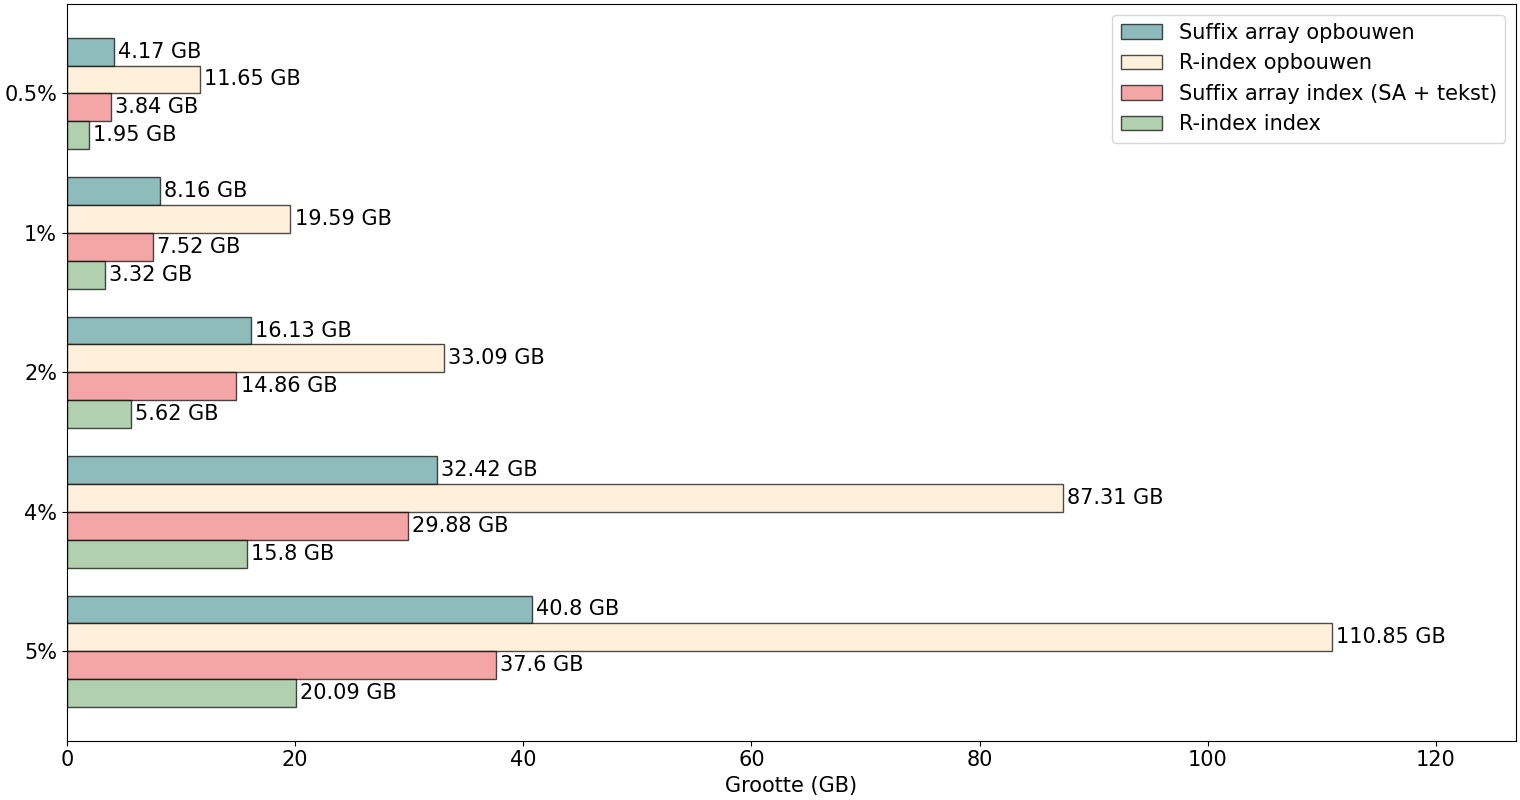
\includegraphics[width=0.8\linewidth]{sa_vs_r_index}
    \caption{Het geheugengebruik tijdens het opbouwen van de suffix array, of R-index en de grootte van de resulterende index. De index wordt opgebouwd voor verschillende subsets van UniProtKB. In elke test gaat het om de eerst $x$ procent van de database. Bij suffix arrays sparseness factor $k = 1$ gebruikt. Indien een andere factor gebruikt zou worden, heeft dit enkel invloed op de grootte van de resulterende index.}
    \label{fig:sa_vs_r_index}
\end{figure}

